\input{preamble.tex}

\begin{document}

\begin{center}
    \textbf{\Large ΛΥΣΕΙΣ ΘΕΜΑΤΩΝ ΣΕΠΤΕΜΒΡΙΟΥ 2022}
\end{center}

\begin{thema}[label=\bf\large{ΘΕΜΑ \textcolor{black}{\arabic*}}]

\item % ΘΕΜΑ 1
\textbf{Δίνεται η ακολουθία με ν-οστό όρο:} $a_n = \frac{1}{n+1} + \frac{1}{n+2} + \dots + \frac{1}{2n}$.

\begin{alist}
    \item \textbf{Γράψτε τους τρεις πρώτους όρους της.}
    
    Για $n=1$:
    \[ a_1 = \frac{1}{1+1} = \frac{1}{2} \]
    
    Για $n=2$:
    \[ a_2 = \frac{1}{2+1} + \frac{1}{2+2} = \frac{1}{3} + \frac{1}{4} = \frac{4+3}{12} = \frac{7}{12} \]
    
    Για $n=3$:
    \[ a_3 = \frac{1}{3+1} + \frac{1}{3+2} + \frac{1}{3+3} = \frac{1}{4} + \frac{1}{5} + \frac{1}{6} = \frac{15+12+10}{60} = \frac{37}{60} \]

    \item \textbf{Αποδείξτε ότι έχει όριο.}
    
    Θα εξετάσουμε τη μονοτονία της ακολουθίας. Υπολογίζουμε τη διαφορά $a_{n+1} - a_n$:
    \[ a_{n+1} = \frac{1}{n+2} + \dots + \frac{1}{2n} + \frac{1}{2n+1} + \frac{1}{2n+2} \]
    \[ a_n = \frac{1}{n+1} + \frac{1}{n+2} + \dots + \frac{1}{2n} \]
    Αφαιρώντας κατά μέλη:
    \[ a_{n+1} - a_n = \frac{1}{2n+1} + \frac{1}{2n+2} - \frac{1}{n+1} \]
    \[ = \frac{1}{2n+1} + \frac{1}{2(n+1)} - \frac{2}{2(n+1)} = \frac{1}{2n+1} - \frac{1}{2n+2} \]
    \[ = \frac{2n+2 - (2n+1)}{(2n+1)(2n+2)} = \frac{1}{(2n+1)(2n+2)} > 0 \]
    Άρα η $a_n$ είναι γνησίως αύξουσα.
    
    Επίσης, η ακολουθία είναι φραγμένη. Έχουμε $n$ όρους, όπου ο μεγαλύτερος είναι ο πρώτος ($\frac{1}{n+1}$) και ο μικρότερος ο τελευταίος ($\frac{1}{2n}$).
    \[ a_n < n \cdot \frac{1}{n+1} = \frac{n}{n+1} < 1 \]
    Επομένως, $a_n < 1$ για κάθε $n$.
    Αφού η $a_n$ είναι γνησίως αύξουσα και άνω φραγμένη, συγκλίνει σε πραγματικό αριθμό.
\end{alist}

\item % ΘΕΜΑ 2
\textbf{Να εξετάσετε ως προς την σύγκλιση τις παρακάτω σειρές:}

\begin{rlist}
    \item $\displaystyle \sum_{n=1}^{\infty} \frac{(n+1)(n+2)}{n!}$
    
    Χρησιμοποιούμε το Κριτήριο Λόγου (\eng{D'Alembert}):
    \[ \frac{a_{n+1}}{a_n} = \frac{(n+2)(n+3)}{(n+1)!} \cdot \frac{n!}{(n+1)(n+2)} = \frac{n+3}{(n+1)^2} \]
    \[ \lim_{n\to\infty} \frac{n+3}{n^2+2n+1} = 0 < 1 \]
    Άρα η σειρά συγκλίνει.

    \item $\displaystyle \sum_{n=1}^{\infty} \frac{5^{n-1}}{n 4^n} = \sum_{n=1}^{\infty} \frac{1}{5n} \left(\frac{5}{4}\right)^n$
    
    Εφαρμόζουμε το Κριτήριο Λόγου:
    \[ \frac{a_{n+1}}{a_n} = \frac{\frac{1}{5(n+1)}(\frac{5}{4})^{n+1}}{\frac{1}{5n}(\frac{5}{4})^n} = \frac{n}{n+1} \cdot \frac{5}{4} \to 1 \cdot \frac{5}{4} = \frac{5}{4} > 1 \]
    Άρα η σειρά αποκλίνει.
\end{rlist}

\item % ΘΕΜΑ 3
\textbf{Να υπολογίσετε τα παρακάτω όρια:}

\begin{rlist}
    \item $\displaystyle \lim_{x\to 0} (\cos x)^{1/x}$
    
    Έστω $y = (\cos x)^{1/x}$. Τότε $\ln y = \frac{\ln(\cos x)}{x}$.
    Πρόκειται για μορφή $0/0$. Εφαρμόζουμε \eng{De L' Hospital}:
    \[ \lim_{x\to 0} \frac{(\ln(\cos x))'}{(x)'} = \lim_{x\to 0} \frac{\frac{-\sin x}{\cos x}}{1} = \lim_{x\to 0} (-\tan x) = 0 \]
    Άρα $\ln y \to 0 \implies y \to e^0 = 1$.

    \item $\displaystyle \lim_{x\to 0} \frac{\arctan x}{\arcsin x}$
    
    Μορφή $0/0$. Εφαρμόζουμε \eng{De L' Hospital}:
    \[ \lim_{x\to 0} \frac{(\arctan x)'}{(\arcsin x)'} = \lim_{x\to 0} \frac{\frac{1}{1+x^2}}{\frac{1}{\sqrt{1-x^2}}} = \frac{1}{1} = 1 \]

    \item $\displaystyle \lim_{x\to \infty} \frac{x^2+x-1}{e^x + e^{-x}}$
    
    Μορφή $\infty/\infty$. Εφαρμόζουμε \eng{De L' Hospital} δύο φορές:
    \[ \lim_{x\to \infty} \frac{2x+1}{e^x - e^{-x}} \overset{DLH}{=} \lim_{x\to \infty} \frac{2}{e^x + e^{-x}} = 0 \]
\end{rlist}

\item % ΘΕΜΑ 4
\textbf{Δίνεται η συνάρτηση} $f(x) = \frac{6x^2-6}{x^3}$.

\begin{alist}
    \item \textbf{Σημεία τομής με τους άξονες:}
    Για $y=0 \implies 6x^2-6=0 \implies x=\pm 1$. Σημεία: $(1,0)$ και $(-1,0)$.
    Για $x=0$, η $f$ δεν ορίζεται.

    \item \textbf{Ασύμπτωτες:}
    Κατακόρυφη στο $x=0$:
    $\lim_{x\to 0^+} f(x) = \lim \frac{-6}{0^+} = -\infty$, $\lim_{x\to 0^-} f(x) = +\infty$. Άρα $x=0$ Κ.Α.
    Οριζόντια:
    $\lim_{x\to \pm\infty} \frac{6x^2}{x^3} = \lim \frac{6}{x} = 0$. Άρα $y=0$ Ο.Α.

    \item \textbf{Μονοτονία και Ακρότατα:}
    $f'(x) = \left(6x^{-1} - 6x^{-3}\right)' = -6x^{-2} + 18x^{-4} = \frac{-6x^2+18}{x^4}$.
    $f'(x) = 0 \implies x^2=3 \implies x=\pm\sqrt{3}$.
    Πρόσημο $f'(x)$: Θετικό στο $(-\sqrt{3}, \sqrt{3})$ (εκτός του 0).
    Η $f$ είναι γνησίως φθίνουσα στο $(-\infty, -\sqrt{3}]$ και στο $[\sqrt{3}, \infty)$.
    Γνησίως αύξουσα στο $[-\sqrt{3}, 0)$ και $(0, \sqrt{3}]$.
    Τοπικό ελάχιστο: $f(-\sqrt{3}) = \frac{12}{-3\sqrt{3}} = -\frac{4\sqrt{3}}{3}$.
    Τοπικό μέγιστο: $f(\sqrt{3}) = \frac{4\sqrt{3}}{3}$.

    \item \textbf{Κυρτότητα και Σημεία Καμπής:}
    $f''(x) = (12x^{-3} - 72x^{-5})' \dots$ λάθος παράγωγος παραπάνω (στο πρόχειρο).
    Ας ξαναδούμε: $f'(x) = -6x^{-2} + 18x^{-4}$.
    $f''(x) = 12x^{-3} - 72x^{-5} = \frac{12x^2-72}{x^5}$.
    Ρίζες $f''(x)$: $x^2=6 \implies x=\pm\sqrt{6}$.
    Πρόσημο $f''(x)$:
    $(-\infty, -\sqrt{6})$: $x^2-6>0, x^5<0 \implies (-)$. Κοίλη.
    $(-\sqrt{6}, 0)$: $x^2-6<0, x^5<0 \implies (+)$. Κυρτή.
    $(0, \sqrt{6})$: $x^2-6<0, x^5>0 \implies (-)$. Κοίλη.
    $(\sqrt{6}, \infty)$: $x^2-6>0, x^5>0 \implies (+)$. Κυρτή.
    Σημεία καμπής στα $x=\pm\sqrt{6}$.

    \item \textbf{Γραφική Παράσταση:}
    \begin{center}
    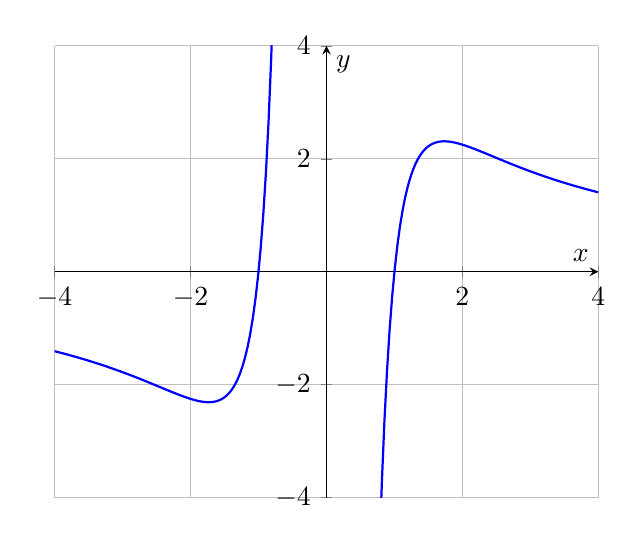
\begin{tikzpicture}
    \begin{axis}[
        axis lines=middle,
        xmin=-4, xmax=4,
        ymin=-4, ymax=4,
        xlabel=$x$, ylabel=$y$,
        restrict y to domain=-10:10,
        samples=100,
        grid=major,
        width=0.7\linewidth,
    ]
    \addplot[blue, thick, domain=-4:-0.2] { (6*x^2-6)/x^3 };
    \addplot[blue, thick, domain=0.2:4] { (6*x^2-6)/x^3 };
    \end{axis}
    \end{tikzpicture}
    \end{center}
\end{alist}

\item % ΘΕΜΑ 5
\textbf{Να υπολογιστούν τα ολοκληρώματα:}

\begin{rlist}
    \item $I = \int \sin(\ln x) \, dx$.
    
    Θέτουμε $u = \ln x \implies x = e^u \implies dx = e^u du$.
    \[ I = \int e^u \sin u \, du \]
    Με δύο φορές παραγοντική:
    \[ I = \frac{e^u}{2}(\sin u - \cos u) + c = \frac{x}{2}(\sin(\ln x) - \cos(\ln x)) + c \]

    \item $J = \int \sin^3 x \cos^2 x \, dx = \int \sin^2 x \cos^2 x \sin x \, dx$
    \[ = \int (1-\cos^2 x) \cos^2 x \sin x \, dx \]
    Θέτουμε $u = \cos x \implies du = -\sin x \, dx$.
    \[ J = -\int (1-u^2)u^2 \, du = \int (u^4 - u^2) \, du = \frac{u^5}{5} - \frac{u^3}{3} + c \]
    \[ = \frac{\cos^5 x}{5} - \frac{\cos^3 x}{3} + c \]
\end{rlist}

\end{thema}

\end{document}
